\textbf{4.} Choose a probability density function other than the uniform, exponential or Laplace. 
Verify Chebyshev's inequality in equation (4.18) of the Fourier book with a computer-generated plot
\footnote{In other words, use Excel, MATLAB, or other appropriate software. Not hand drawn.}
of the inequality as a function of $a$. \\
\textbf{Solution:} \\
Chebyshev's inequality:
\begin{align*}
  \int_{\left| x - \ol{X}\leq a\right|}f_X(x)dx & \geq 1 - \left( \df{\sigma_X}{a} \right)^2
\end{align*}

In figure~\ref{fig:cheby}, blue line is a gaussian distribution with $\mu = 0, \sigma = 3$. 
Green line is a function of
\begin{align*}
  S(a) & = \int_{\ol{X} - a}^{\ol{X} + a}f_X(x)dx
\end{align*}
Red line is a function of
\begin{align*}
  Y(a) & = 1 - \left( \df{\sigma_X}{a} \right)^2
\end{align*}

The part for $-\sigma < a < \sigma$ is not shown, since they are negative.

\begin{figure}[h!]
  \begin{center}
    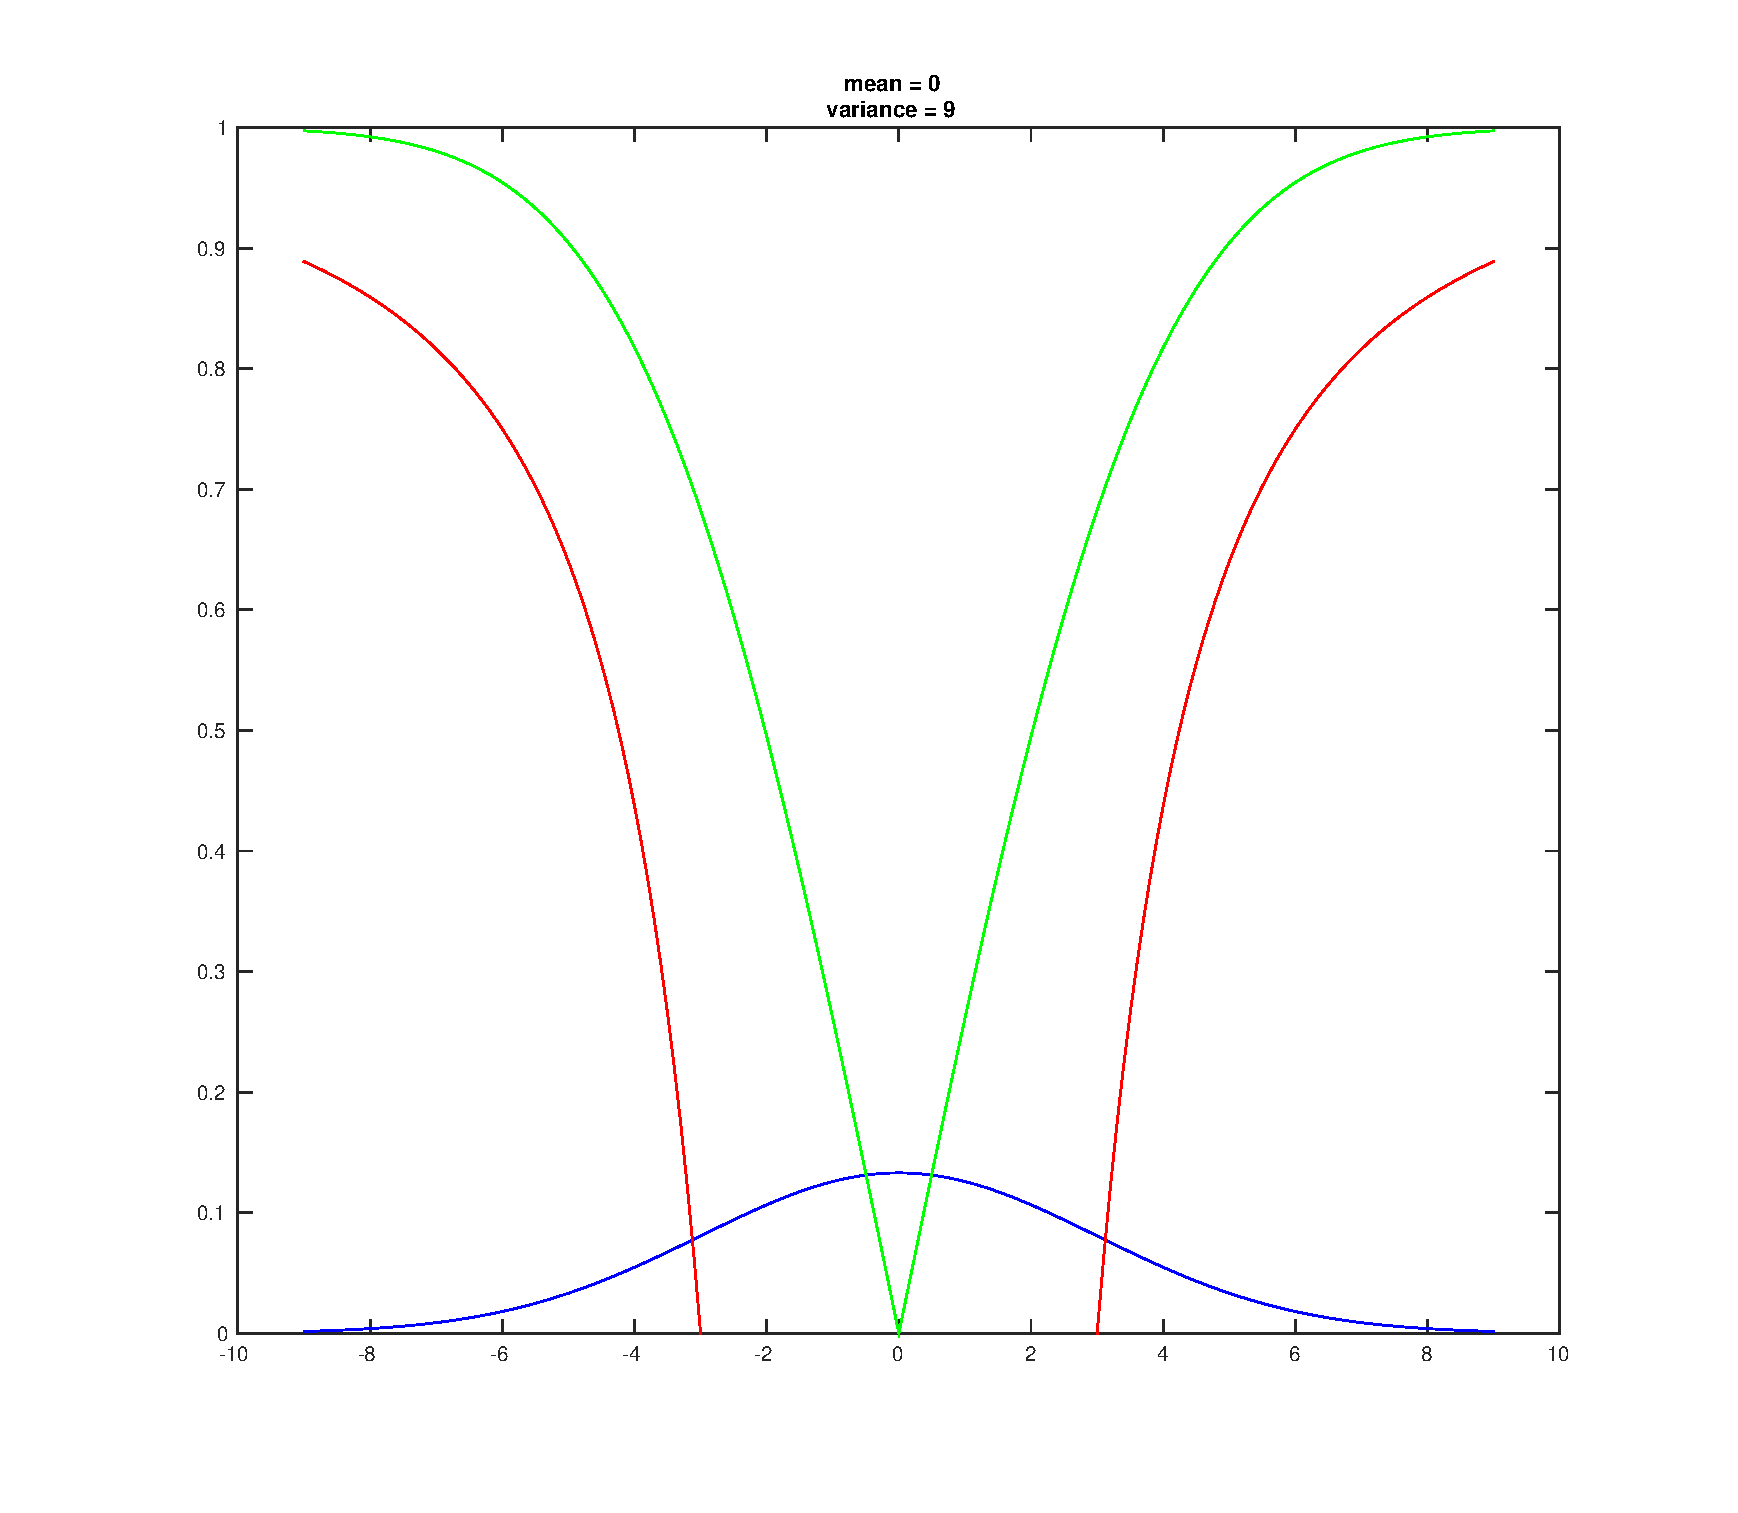
\includegraphics[width=6in]{chebyshev_inequality.eps}
  \end{center}
  \caption{Chebyshev's Inequality}
  \label{fig:cheby}
\end{figure}

\SourceCode{matlab}{Chebyshev's Inequality verification}{lst:p4}{../src/matlab/problem4.m}
\vspace{.5in}
